%
\begin{isabellebody}%
\def\isabellecontext{Introduction}%
%
\isadelimtheory
%
\endisadelimtheory
%
\isatagtheory
\isacommand{theory}\isamarkupfalse%
\ Introduction\isanewline
\isakeyword{imports}\ Setup\isanewline
\isakeyword{begin}%
\endisatagtheory
{\isafoldtheory}%
%
\isadelimtheory
%
\endisadelimtheory
%
\isamarkupchapter{Code generation from \isa{Isabelle{\isacharslash}HOL} theories%
}
\isamarkuptrue%
%
\isamarkupsection{Introduction and Overview%
}
\isamarkuptrue%
%
\begin{isamarkuptext}%
This tutorial introduces a generic code generator for the
  \isa{Isabelle} system.
  Generic in the sense that the
  \qn{target language} for which code shall ultimately be
  generated is not fixed but may be an arbitrary state-of-the-art
  functional programming language (currently, the implementation
  supports \isa{SML} \cite{SML}, \isa{OCaml} \cite{OCaml} and \isa{Haskell}
  \cite{haskell-revised-report}).

  Conceptually the code generator framework is part
  of Isabelle's \hyperlink{theory.Pure}{\mbox{\isa{Pure}}} meta logic framework; the logic
  \hyperlink{theory.HOL}{\mbox{\isa{HOL}}} which is an extension of \hyperlink{theory.Pure}{\mbox{\isa{Pure}}}
  already comes with a reasonable framework setup and thus provides
  a good working horse for raising code-generation-driven
  applications.  So, we assume some familiarity and experience
  with the ingredients of the \hyperlink{theory.HOL}{\mbox{\isa{HOL}}} distribution theories.
  (see also \cite{isa-tutorial}).

  The code generator aims to be usable with no further ado
  in most cases while allowing for detailed customisation.
  This manifests in the structure of this tutorial: after a short
  conceptual introduction with an example (\secref{sec:intro}),
  we discuss the generic customisation facilities (\secref{sec:program}).
  A further section (\secref{sec:adaption}) is dedicated to the matter of
  \qn{adaption} to specific target language environments.  After some
  further issues (\secref{sec:further}) we conclude with an overview
  of some ML programming interfaces (\secref{sec:ml}).

  \begin{warn}
    Ultimately, the code generator which this tutorial deals with
    is supposed to replace the existing code generator
    by Stefan Berghofer \cite{Berghofer-Nipkow:2002}.
    So, for the moment, there are two distinct code generators
    in Isabelle.  In case of ambiguity, we will refer to the framework
    described here as \isa{generic\ code\ generator}, to the
    other as \isa{SML\ code\ generator}.
    Also note that while the framework itself is
    object-logic independent, only \hyperlink{theory.HOL}{\mbox{\isa{HOL}}} provides a reasonable
    framework setup.    
  \end{warn}%
\end{isamarkuptext}%
\isamarkuptrue%
%
\isamarkupsubsection{Code generation via shallow embedding \label{sec:intro}%
}
\isamarkuptrue%
%
\begin{isamarkuptext}%
The key concept for understanding \isa{Isabelle}'s code generation is
  \emph{shallow embedding}, i.e.~logical entities like constants, types and
  classes are identified with corresponding concepts in the target language.

  Inside \hyperlink{theory.HOL}{\mbox{\isa{HOL}}}, the \hyperlink{command.datatype}{\mbox{\isa{\isacommand{datatype}}}} and
  \hyperlink{command.definition}{\mbox{\isa{\isacommand{definition}}}}/\hyperlink{command.primrec}{\mbox{\isa{\isacommand{primrec}}}}/\hyperlink{command.fun}{\mbox{\isa{\isacommand{fun}}}} declarations form
  the core of a functional programming language.  The default code generator setup
  allows to turn those into functional programs immediately.
  This means that \qt{naive} code generation can proceed without further ado.
  For example, here a simple \qt{implementation} of amortised queues:%
\end{isamarkuptext}%
\isamarkuptrue%
%
\isadelimquote
%
\endisadelimquote
%
\isatagquote
\isacommand{datatype}\isamarkupfalse%
\ {\isacharprime}a\ queue\ {\isacharequal}\ Queue\ {\isachardoublequoteopen}{\isacharprime}a\ list{\isachardoublequoteclose}\ {\isachardoublequoteopen}{\isacharprime}a\ list{\isachardoublequoteclose}\isanewline
\isanewline
\isacommand{definition}\isamarkupfalse%
\ empty\ {\isacharcolon}{\isacharcolon}\ {\isachardoublequoteopen}{\isacharprime}a\ queue{\isachardoublequoteclose}\ \isakeyword{where}\isanewline
\ \ {\isachardoublequoteopen}empty\ {\isacharequal}\ Queue\ {\isacharbrackleft}{\isacharbrackright}\ {\isacharbrackleft}{\isacharbrackright}{\isachardoublequoteclose}\isanewline
\isanewline
\isacommand{primrec}\isamarkupfalse%
\ enqueue\ {\isacharcolon}{\isacharcolon}\ {\isachardoublequoteopen}{\isacharprime}a\ {\isasymRightarrow}\ {\isacharprime}a\ queue\ {\isasymRightarrow}\ {\isacharprime}a\ queue{\isachardoublequoteclose}\ \isakeyword{where}\isanewline
\ \ {\isachardoublequoteopen}enqueue\ x\ {\isacharparenleft}Queue\ xs\ ys{\isacharparenright}\ {\isacharequal}\ Queue\ {\isacharparenleft}x\ {\isacharhash}\ xs{\isacharparenright}\ ys{\isachardoublequoteclose}\isanewline
\isanewline
\isacommand{fun}\isamarkupfalse%
\ dequeue\ {\isacharcolon}{\isacharcolon}\ {\isachardoublequoteopen}{\isacharprime}a\ queue\ {\isasymRightarrow}\ {\isacharprime}a\ option\ {\isasymtimes}\ {\isacharprime}a\ queue{\isachardoublequoteclose}\ \isakeyword{where}\isanewline
\ \ \ \ {\isachardoublequoteopen}dequeue\ {\isacharparenleft}Queue\ {\isacharbrackleft}{\isacharbrackright}\ {\isacharbrackleft}{\isacharbrackright}{\isacharparenright}\ {\isacharequal}\ {\isacharparenleft}None{\isacharcomma}\ Queue\ {\isacharbrackleft}{\isacharbrackright}\ {\isacharbrackleft}{\isacharbrackright}{\isacharparenright}{\isachardoublequoteclose}\isanewline
\ \ {\isacharbar}\ {\isachardoublequoteopen}dequeue\ {\isacharparenleft}Queue\ xs\ {\isacharparenleft}y\ {\isacharhash}\ ys{\isacharparenright}{\isacharparenright}\ {\isacharequal}\ {\isacharparenleft}Some\ y{\isacharcomma}\ Queue\ xs\ ys{\isacharparenright}{\isachardoublequoteclose}\isanewline
\ \ {\isacharbar}\ {\isachardoublequoteopen}dequeue\ {\isacharparenleft}Queue\ xs\ {\isacharbrackleft}{\isacharbrackright}{\isacharparenright}\ {\isacharequal}\isanewline
\ \ \ \ \ \ {\isacharparenleft}case\ rev\ xs\ of\ y\ {\isacharhash}\ ys\ {\isasymRightarrow}\ {\isacharparenleft}Some\ y{\isacharcomma}\ Queue\ {\isacharbrackleft}{\isacharbrackright}\ ys{\isacharparenright}{\isacharparenright}{\isachardoublequoteclose}%
\endisatagquote
{\isafoldquote}%
%
\isadelimquote
%
\endisadelimquote
%
\begin{isamarkuptext}%
\noindent Then we can generate code e.g.~for \isa{SML} as follows:%
\end{isamarkuptext}%
\isamarkuptrue%
%
\isadelimquote
%
\endisadelimquote
%
\isatagquote
\isacommand{export{\isacharunderscore}code}\isamarkupfalse%
\ empty\ dequeue\ enqueue\ \isakeyword{in}\ SML\isanewline
\ \ \isakeyword{module{\isacharunderscore}name}\ Example\ \isakeyword{file}\ {\isachardoublequoteopen}examples{\isacharslash}example{\isachardot}ML{\isachardoublequoteclose}%
\endisatagquote
{\isafoldquote}%
%
\isadelimquote
%
\endisadelimquote
%
\begin{isamarkuptext}%
\noindent resulting in the following code:%
\end{isamarkuptext}%
\isamarkuptrue%
%
\isadelimquote
%
\endisadelimquote
%
\isatagquote
%
\begin{isamarkuptext}%
\isaverbatim%
\noindent%
\verb|structure Example = |\newline%
\verb|struct|\newline%
\newline%
\verb|fun foldl f a [] = a|\newline%
\verb|  |\verb,|,\verb| foldl f a (x :: xs) = foldl f (f a x) xs;|\newline%
\newline%
\verb|fun rev xs = foldl (fn xsa => fn x => x :: xsa) [] xs;|\newline%
\newline%
\verb|fun list_case f1 f2 (a :: lista) = f2 a lista|\newline%
\verb|  |\verb,|,\verb| list_case f1 f2 [] = f1;|\newline%
\newline%
\verb|datatype 'a queue = Queue of 'a list * 'a list;|\newline%
\newline%
\verb|val empty : 'a queue = Queue ([], []);|\newline%
\newline%
\verb|fun dequeue (Queue ([], [])) = (NONE, Queue ([], []))|\newline%
\verb|  |\verb,|,\verb| dequeue (Queue (xs, y :: ys)) = (SOME y, Queue (xs, ys))|\newline%
\verb|  |\verb,|,\verb| dequeue (Queue (v :: va, [])) =|\newline%
\verb|    let|\newline%
\verb|      val y :: ys = rev (v :: va);|\newline%
\verb|    in|\newline%
\verb|      (SOME y, Queue ([], ys))|\newline%
\verb|    end;|\newline%
\newline%
\verb|fun enqueue x (Queue (xs, ys)) = Queue (x :: xs, ys);|\newline%
\newline%
\verb|end; (*struct Example*)|%
\end{isamarkuptext}%
\isamarkuptrue%
%
\endisatagquote
{\isafoldquote}%
%
\isadelimquote
%
\endisadelimquote
%
\begin{isamarkuptext}%
\noindent The \hyperlink{command.export-code}{\mbox{\isa{\isacommand{export{\isacharunderscore}code}}}} command takes a space-separated list of
  constants for which code shall be generated;  anything else needed for those
  is added implicitly.  Then follows a target language identifier
  (\isa{SML}, \isa{OCaml} or \isa{Haskell}) and a freely chosen module name.
  A file name denotes the destination to store the generated code.  Note that
  the semantics of the destination depends on the target language:  for
  \isa{SML} and \isa{OCaml} it denotes a \emph{file}, for \isa{Haskell}
  it denotes a \emph{directory} where a file named as the module name
  (with extension \isa{{\isachardot}hs}) is written:%
\end{isamarkuptext}%
\isamarkuptrue%
%
\isadelimquote
%
\endisadelimquote
%
\isatagquote
\isacommand{export{\isacharunderscore}code}\isamarkupfalse%
\ empty\ dequeue\ enqueue\ \isakeyword{in}\ Haskell\isanewline
\ \ \isakeyword{module{\isacharunderscore}name}\ Example\ \isakeyword{file}\ {\isachardoublequoteopen}examples{\isacharslash}{\isachardoublequoteclose}%
\endisatagquote
{\isafoldquote}%
%
\isadelimquote
%
\endisadelimquote
%
\begin{isamarkuptext}%
\noindent This is how the corresponding code in \isa{Haskell} looks like:%
\end{isamarkuptext}%
\isamarkuptrue%
%
\isadelimquote
%
\endisadelimquote
%
\isatagquote
%
\begin{isamarkuptext}%
\isaverbatim%
\noindent%
\verb|module Example where {|\newline%
\newline%
\newline%
\verb|foldla :: forall a b. (a -> b -> a) -> a -> [b] -> a;|\newline%
\verb|foldla f a [] = a;|\newline%
\verb|foldla f a (x : xs) = foldla f (f a x) xs;|\newline%
\newline%
\verb|rev :: forall a. [a] -> [a];|\newline%
\verb|rev xs = foldla (\ xsa x -> x : xsa) [] xs;|\newline%
\newline%
\verb|list_case :: forall t a. t -> (a -> [a] -> t) -> [a] -> t;|\newline%
\verb|list_case f1 f2 (a : list) = f2 a list;|\newline%
\verb|list_case f1 f2 [] = f1;|\newline%
\newline%
\verb|data Queue a = Queue [a] [a];|\newline%
\newline%
\verb|empty :: forall a. Queue a;|\newline%
\verb|empty = Queue [] [];|\newline%
\newline%
\verb|dequeue :: forall a. Queue a -> (Maybe a, Queue a);|\newline%
\verb|dequeue (Queue [] []) = (Nothing, Queue [] []);|\newline%
\verb|dequeue (Queue xs (y : ys)) = (Just y, Queue xs ys);|\newline%
\verb|dequeue (Queue (v : va) []) =|\newline%
\verb|  let {|\newline%
\verb|    (y : ys) = rev (v : va);|\newline%
\verb|  } in (Just y, Queue [] ys);|\newline%
\newline%
\verb|enqueue :: forall a. a -> Queue a -> Queue a;|\newline%
\verb|enqueue x (Queue xs ys) = Queue (x : xs) ys;|\newline%
\newline%
\verb|}|%
\end{isamarkuptext}%
\isamarkuptrue%
%
\endisatagquote
{\isafoldquote}%
%
\isadelimquote
%
\endisadelimquote
%
\begin{isamarkuptext}%
\noindent This demonstrates the basic usage of the \hyperlink{command.export-code}{\mbox{\isa{\isacommand{export{\isacharunderscore}code}}}} command;
  for more details see \secref{sec:further}.%
\end{isamarkuptext}%
\isamarkuptrue%
%
\isamarkupsubsection{Code generator architecture \label{sec:concept}%
}
\isamarkuptrue%
%
\begin{isamarkuptext}%
What you have seen so far should be already enough in a lot of cases.  If you
  are content with this, you can quit reading here.  Anyway, in order to customise
  and adapt the code generator, it is inevitable to gain some understanding
  how it works.

  \begin{figure}[h]
    \centering
    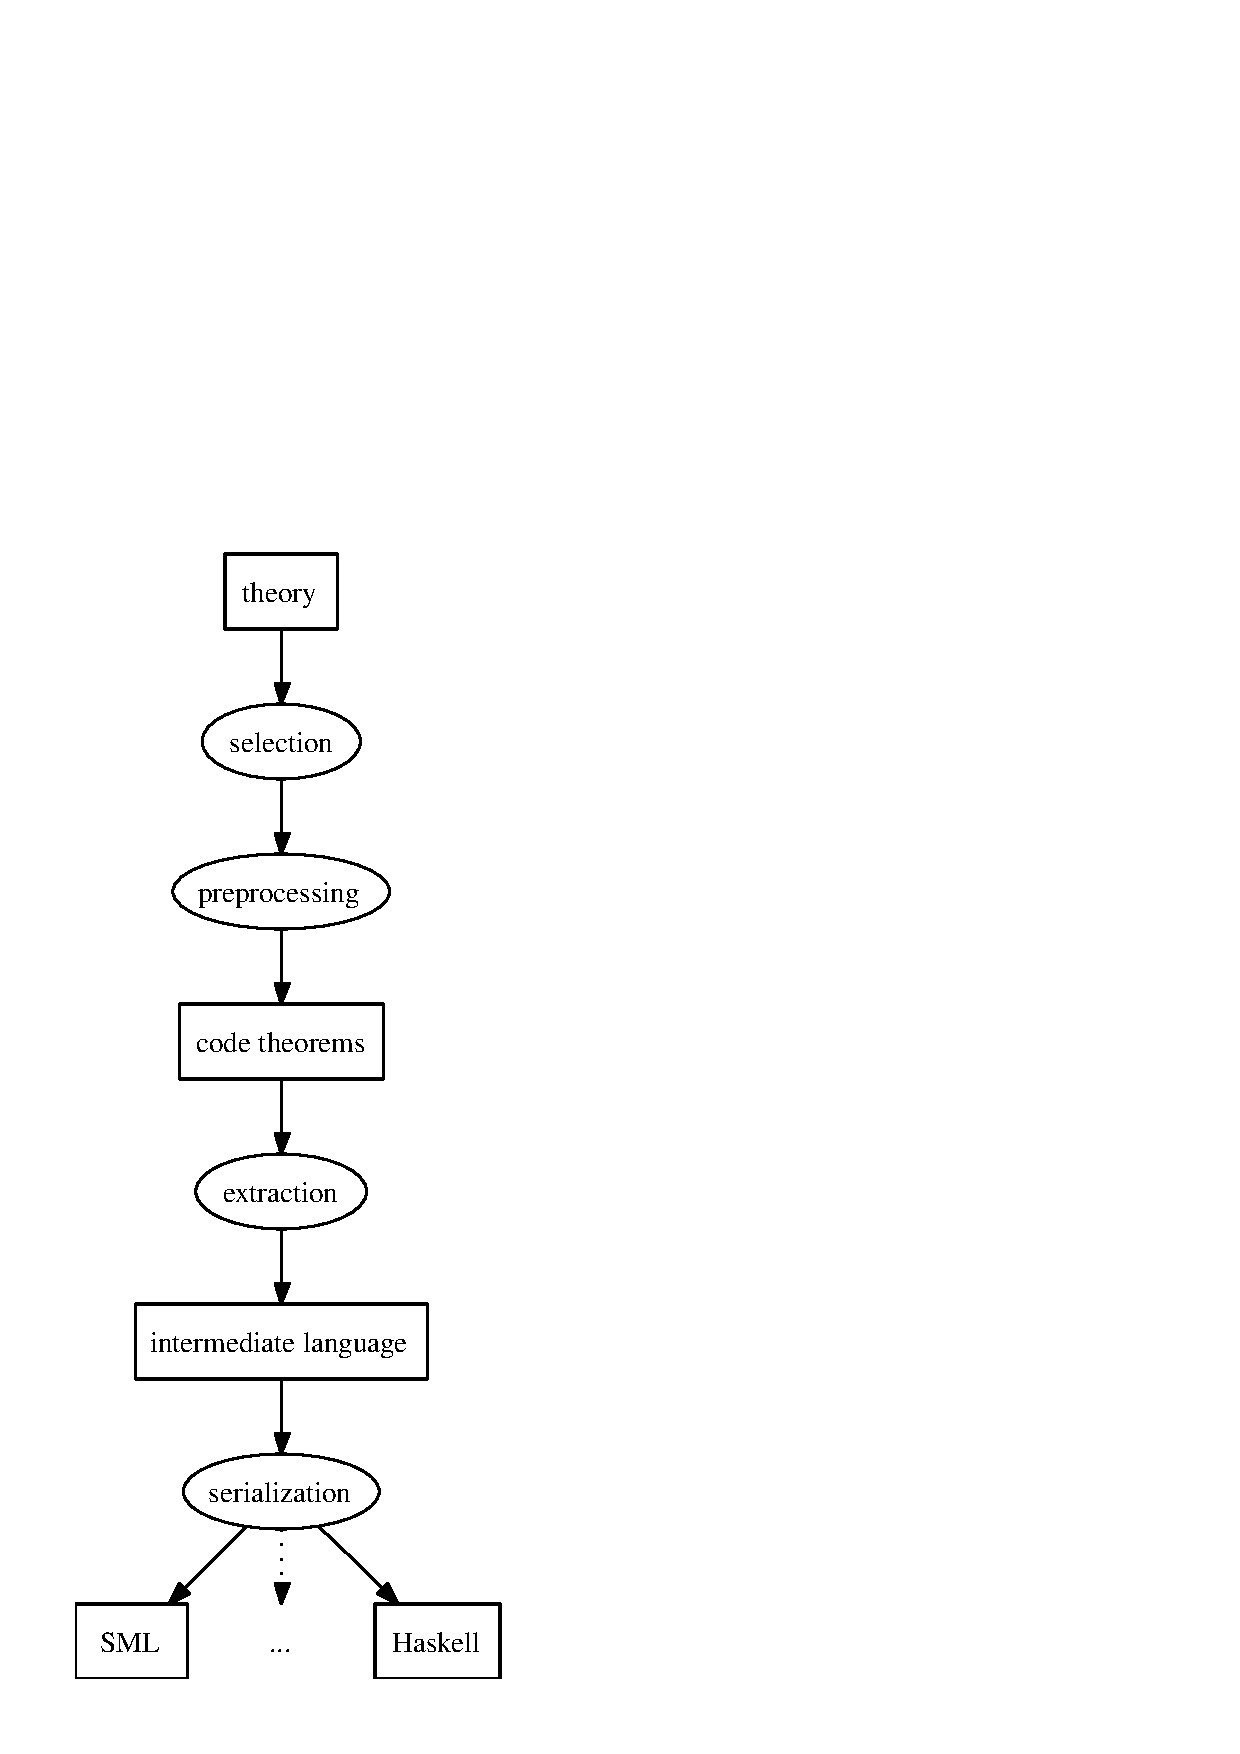
\includegraphics[width=0.7\textwidth]{codegen_process}
    \caption{Code generator architecture}
    \label{fig:arch}
  \end{figure}

  The code generator employs a notion of executability
  for three foundational executable ingredients known
  from functional programming:
  \emph{defining equations}, \emph{datatypes}, and
  \emph{type classes}.  A defining equation as a first approximation
  is a theorem of the form \isa{f\ t\isactrlisub {\isadigit{1}}\ t\isactrlisub {\isadigit{2}}\ {\isasymdots}\ t\isactrlisub n\ {\isasymequiv}\ t}
  (an equation headed by a constant \isa{f} with arguments
  \isa{t\isactrlisub {\isadigit{1}}\ t\isactrlisub {\isadigit{2}}\ {\isasymdots}\ t\isactrlisub n} and right hand side \isa{t}).
  Code generation aims to turn defining equations
  into a functional program.  This is achieved by three major
  components which operate sequentially, i.e. the result of one is
  the input
  of the next in the chain,  see diagram \ref{fig:arch}:

  \begin{itemize}

    \item Out of the vast collection of theorems proven in a
      \qn{theory}, a reasonable subset modelling
      defining equations is \qn{selected}.

    \item On those selected theorems, certain
      transformations are carried out
      (\qn{preprocessing}).  Their purpose is to turn theorems
      representing non- or badly executable
      specifications into equivalent but executable counterparts.
      The result is a structured collection of \qn{code theorems}.

    \item Before the selected defining equations are continued with,
      they can be \qn{preprocessed}, i.e. subjected to theorem
      transformations.  This \qn{preprocessor} is an interface which
      allows to apply
      the full expressiveness of ML-based theorem transformations
      to code generation;  motivating examples are shown below, see
      \secref{sec:preproc}.
      The result of the preprocessing step is a structured collection
      of defining equations.

    \item These defining equations are \qn{translated} to a program
      in an abstract intermediate language.  Think of it as a kind
      of \qt{Mini-Haskell} with four \qn{statements}: \isa{data}
      (for datatypes), \isa{fun} (stemming from defining equations),
      also \isa{class} and \isa{inst} (for type classes).

    \item Finally, the abstract program is \qn{serialised} into concrete
      source code of a target language.

  \end{itemize}

  \noindent From these steps, only the two last are carried out outside the logic;  by
  keeping this layer as thin as possible, the amount of code to trust is
  kept to a minimum.%
\end{isamarkuptext}%
\isamarkuptrue%
%
\isadelimtheory
%
\endisadelimtheory
%
\isatagtheory
\isacommand{end}\isamarkupfalse%
%
\endisatagtheory
{\isafoldtheory}%
%
\isadelimtheory
%
\endisadelimtheory
\isanewline
\end{isabellebody}%
%%% Local Variables:
%%% mode: latex
%%% TeX-master: "root"
%%% End:
